\documentclass[12pt]{article}
\usepackage{geometry}                % See geometry.pdf to learn the layout options. There are lots.
\geometry{letterpaper}                   % ... or a4paper or a5paper or ... 
%\geometry{landscape}                % Activate for for rotated page geometry
\usepackage[parfill]{parskip}    % Activate to begin paragraphs with an empty line rather than an indent
\usepackage{daves,fancyhdr,natbib,graphicx,dcolumn,amsmath,lastpage,url}
\usepackage{amsmath,amssymb,epstopdf,longtable}
\usepackage{paralist}  % need to properly formulate standard answer blocks
\usepackage[final]{pdfpages}
\DeclareGraphicsRule{.tif}{png}{.png}{`convert #1 `dirname #1`/`basename #1 .tif`.png}
\pagestyle{fancy}
\lhead{CE 3305 Fluid Mechanics; Exercise Set 15}
\rhead{Name:\_\_\_\_\_\_\_\_\_\_\_\_\_\_\_\_\_\_\_\_\_\_\_\_\_\_\_\_\_\_\_\_\_\_}
\lfoot{REVISION A}
\cfoot{}
\rfoot{Page \thepage\ of \pageref{LastPage}}
\renewcommand\headrulewidth{0pt}
%%%%%%%%%%%%%%%%%%%%%%%%%%%%%%%%%%%%
\begin{document}
%%%%%%%%%%%%%%%%%%%%%%%%%%%%%%%%%%%
\begingroup
\begin{center}
{\textbf{{ CE 3305 Engineering Fluid Mechanics} \\ Exercise Set 15 \\ Summer 2018 -- GERMANY} }
\end{center}
\endgroup
\begingroup
~\newline

\begin{enumerate}
\item (Problem 7.56 pg 286)  Figure \ref{fig:Hydropower} is a schematic of a hydropower system.
The elevation difference between the reservoir water surface and the pond water surface downstream of the reservoir (called the tailwater), $H$, is 24 $m$.
The velocity of the water exiting into the pond is 7 $m/s$, and the discharge through the system is 4 $m^3/s$.
Neglect frictional losses in the penstock (the pipe from the reservoir to the turbine).   Estimate the power produced by the turbine in kilowatts.

\begin{figure}[h!] %  figure placement: here, top, bottom, or page
   \centering
   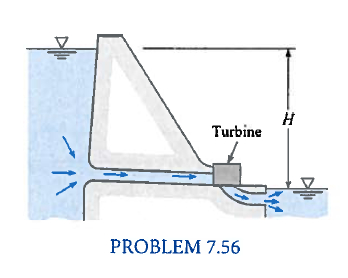
\includegraphics[width=2in]{Hydropower.jpg} 
   \caption{Hydropower system}
   \label{fig:Hydropower}
\end{figure}
\clearpage
(Problem 7.56 pg 286)  (Continued)
\clearpage

\item (Problem 7.87 pg 290) (SI converted from actual problem) 
Figure \ref{fig:PumpUphill} is a schematic of a pumped-storage system.
How much power must be supplied to the water by the pump (in kilowatts) to pump water at 0.085 $m^3/s$ at 20 $^oC$ from the lower to the upper reservoir?\\
~\\
The head loss in the pipes is $h_l=0.018\frac{L}{D}\frac{V^2}{2g}$, where $L$ is the length of the pipe in meters, and $D$ is the diameter of the pipe in meters.
Sketch the HGL and EGL for the system.

\begin{figure}[h!] %  figure placement: here, top, bottom, or page
   \centering
   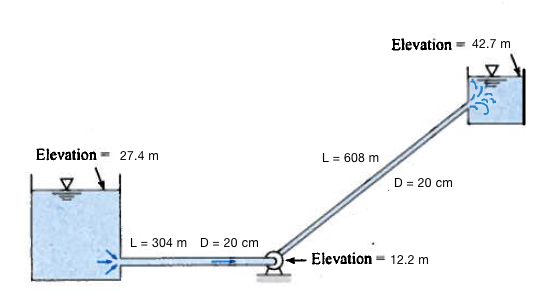
\includegraphics[width=4in]{PumpUphill.jpg} 
   \caption{Pump-storage system}
   \label{fig:PumpUphill}
\end{figure}
\clearpage
 (Problem 7.87 pg 290) (Continued)
\end{enumerate}
\end{document}  